\documentclass[11pt]{ctexart}
\usepackage[top=2cm, bottom=2cm, left=2cm, right=2cm]{geometry}
\usepackage{algorithm,algpseudocode,float}
\makeatletter
\newenvironment{breakablealgorithm}
  {% \begin{breakablealgorithm}
   \begin{center}
     \refstepcounter{algorithm}% New algorithm
     \hrule height.8pt depth0pt \kern2pt% \@fs@pre for \@fs@ruled
     \renewcommand{\caption}[2][\relax]{% Make a new \caption
       {\raggedright\textbf{\ALG@name~\thealgorithm} ##2\par}%
       \ifx\relax##1\relax % #1 is \relax
         \addcontentsline{loa}{algorithm}{\protect\numberline{\thealgorithm}##2}%
       \else % #1 is not \relax
         \addcontentsline{loa}{algorithm}{\protect\numberline{\thealgorithm}##1}%
       \fi
       \kern2pt\hrule\kern2pt
     }
  }{% \end{breakablealgorithm}
     \kern2pt\hrule\relax% \@fs@post for \@fs@ruled
   \end{center}
  }
\makeatother

\usepackage{amsmath}
\usepackage{graphicx}
\usepackage{listings}
\usepackage{xcolor}
\usepackage{float}
\usepackage{amsmath}
\usepackage{amssymb}
\floatname{algorithm}{算法}
\renewcommand{\algorithmicrequire}{\textbf{输入:}}
\renewcommand{\algorithmicensure}{\textbf{输出:}}
\lstset{numbers=left, %设置行号位置
        numberstyle=\tiny, %设置行号大小
        keywordstyle=\color{blue}, %设置关键字颜色
        commentstyle=\color[cmyk]{1,0,1,0}, %设置注释颜色
        frame=single, %设置边框格式
        escapeinside=``, %逃逸字符(1左面的键),用于显示中文
        breaklines, %自动折行
        extendedchars=false, %解决代码跨页时,章节标题,页眉等汉字不显示的问题
        xleftmargin=2em,xrightmargin=2em, aboveskip=1em, %设置边距
        tabsize=4, %设置tab空格数
        showspaces=false %不显示空格
}
\title{\huge\bf
0-1背包 - 实验报告}
\author{毛圆鑫 - 201721012271}
\date{Nov 10, 2019}

\begin{document}  
\maketitle
\section*{说明}
本次代码不长,所以本文以完整的形式给出,但也请见所附的.cpp文件,

还有就是本文档是使用latex语言编写的,其源文件也可见于附件或Github,或https://github.com/punk-boy/algorithm/下的 knapsack.cpp

本次的动态规划问题,主要检查的逻辑的正确性,以及动态规划过程的理解,所以这次代码的测试用例为了简单化,均使用和老师一样的示例。



\section{伪代码}
\begin{breakablealgorithm}
\caption{0-1背包问题 - 动态规划解法 - 伪代码}
\begin{algorithmic}[1]
\Require 价值$v[]$,重量$w[]$,容量$c$,物品种类$n$
\Ensure 背包所能容纳物品的最大价值
\Function {Knapsack}{$v[], w[], c, n$}
\State $jMax=\min(w[n]-1,c)$
\For{$j=0 \to jMax$}
	\State $m[n][j]\gets 0$
\EndFor
\For{$j=w[n] \to c$}
	\State $m[n] \gets v[n]$
\EndFor
\For{$i=n-1 \to 2$}
	\State $jMax\gets \min(w[i]-1, c)$
	\For{$j=0 \to jMax$}
		\State $m[i][j]\gets m[i+1][j]$
	\EndFor
	\For{$j=w[i] \to c$}
		\State $m[i][j]\gets \max(m[i+1][j],m[i+1][j-w[i]]+v[i])$
	\EndFor
\EndFor
\State $m[1][c] \gets m[2][c]$
\If{$c \geqslant w[1]$}
	\State $m[1][c]=\max(m[1][c],m[2][c-w[i]]+v[1])$
\EndIf
\State{\Return $m[1][c]$}
\EndFunction
\end{algorithmic}
\end{breakablealgorithm}


\section{实现代码}
\begin{lstlisting}[language=C++]
#include <stdio.h>
#include <iostream>
#include <string.h>

#define N 100
int dp[N][N];

inline int max(int a, int b)
{
	return a>b?a:b;
}

inline int min(int a, int b)
{
	return a<b?a:b;
}
int knapsack(int * v, int * w, int c, int n)
{
	int jmax = min(w[n-1]-1, c);
	for(int j=0;j<=jmax;j++)
		dp[n-1][j] = 0;
	for(int j=w[n-1];j<=c;j++)
		dp[n-1][j] = v[n-1];	
	for(int i=n-2;i>=1;i--)
	{
		int jMax = min(w[i]-1, c);
		for(int j=0;j<jMax;j++)
			dp[i][j] = dp[i+1][j];
		for(int j=w[i];j<=c;j++)
			dp[i][j] = max(dp[i+1][j],dp[i+1][j-w[i]]+v[i]);
	}
	dp[0][c] = dp[1][c];
	if(c >= w[1])
		dp[0][c] = max(dp[0][c], dp[1][c-w[0]]+v[0]);
	return dp[0][c];
}

int main()
{
	int n = 4;
	int c = 9;
	int w[N] = {2, 3, 4, 5};
	int v[N] = {3, 4, 5, 7};
	int ret = knapsack(v, w, c, n);
	printf("%d\n", ret);
	return 0;
}
\end{lstlisting}

\section{实验结果}
\begin{figure}[H]
\centering
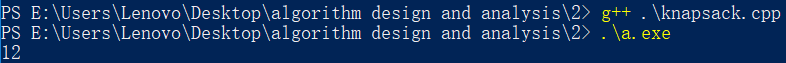
\includegraphics[scale=1.0]{knapsack.png}
\caption{0-1背包实验结果}
\end{figure}

\end{document}



